\section{Impedances}

In a particle accelerator there are a large number of components that have frequency dependent properties, either due to their geometry (for example resonant cavity structures) or material properties (frequency dependent permetivitty/permeability in devices, for example ferrite in normal conducting kicker magnets). In addition many instability mechanisms are strongly modal in nature, thus a frequency analysis of the possible sources of impedance is incredibly valuable. 

\subsection{Beam Coupling Impedance}

The longitudinal beam coupling impedance $Z_{\parallel}$ and the transverse beam coupling impedance $Z_{\perp}$ are defined as the Fourier transforms of the single particle wake function, given by

\begin{align}
Z_{\parallel} \left(\mathbf{r_{1}}, \mathbf{r_{2}}, \omega  \right) = \int^{\infty}_{0} d\tau w_{\parallel} \left(\mathbf{r_{1}}, \mathbf{r_{2}}, \tau  \right) e^{-j\omega \tau}\\
Z_{\perp} \left(\mathbf{r_{1}}, \mathbf{r_{2}}, \omega  \right) = j \int^{\infty}_{0} d\tau w_{\perp} \left(\mathbf{r_{1}}, \mathbf{r_{2}}, \tau  \right) e^{-j\omega \tau} \label{eqn:total_trans_imp}
\end{align}

where $\omega = 2\pi / \tau$. In a similar way the bunch wake function can be related to the longitudinal and transverse beam coupling impedance by considering the Fourier transform of the time dependent bunch current $\lambda \left( \omega  \right) = \int^{\infty}_{-\infty} d\tau i_{b}\left( \tau \right) e^{-j \omega \tau}$, which allows it to be shown that

\begin{align}
W_{\parallel}  \left( \mathbf{r_{2}}, \tau \right) = \int^{\infty}_{- \infty} d \omega Z_{\parallel} \left(\mathbf{r_{1}}, \mathbf{r_{2}}, \omega  \right) \lambda \left( \omega  \right) e^{-j \omega \tau} \\
W_{\perp}  \left( \mathbf{r_{2}}, \tau \right) = \int^{\infty}_{- \infty} d \omega Z_{\perp} \left(\mathbf{r_{1}}, \mathbf{r_{2}}, \omega  \right) \lambda \left( \omega  \right) e^{-j \omega \tau}.
\end{align}

\subsection{Transverse Impedances}

As can be seen in Eqn.~\ref{eqn:total_trans_imp}, the transverse impedance is dependent on the displacement of both the source and witness particles. For reasons of simplifying beam dynamics evaluation, it is useful to distinguish the components dependent only on the transverse displacement of the source particle and that of the witness particle in the vertical and horizontal planes of the beam. This involves seperating the impedance firstly into horizontal and vertical components, and subsequently into components dependent only on the displacement of the source and of the witness particle. These are called the dipolar, or driving impedance and the quadrupolar, or detuning impedance respectively. In addition it can be shown that constant transverse terms exist which must also be taken into account. These are given by

\begin{align}
Z_{\perp, x} \left( x_{1}, x_{2}, \omega \right) &= Z_{dip, x} \left( \omega, x_{1}  \right) +  Z_{quad, x} \left( \omega, x_{2}  \right) + Z_{const, x} \left( \omega  \right) \\
Z_{\perp, y} \left( y_{1}, y_{2}, \omega \right) &= Z_{dip, y} \left( \omega, y_{1}  \right) +  Z_{quad, y} \left( \omega, y_{2}  \right) + Z_{const, y} \left( \omega  \right).
\end{align}

The relative displacements of the source and witness particle are shown in Fig.~\ref{fig:trans_imp_disp} for clarity.

\begin{figure}
\begin{center}
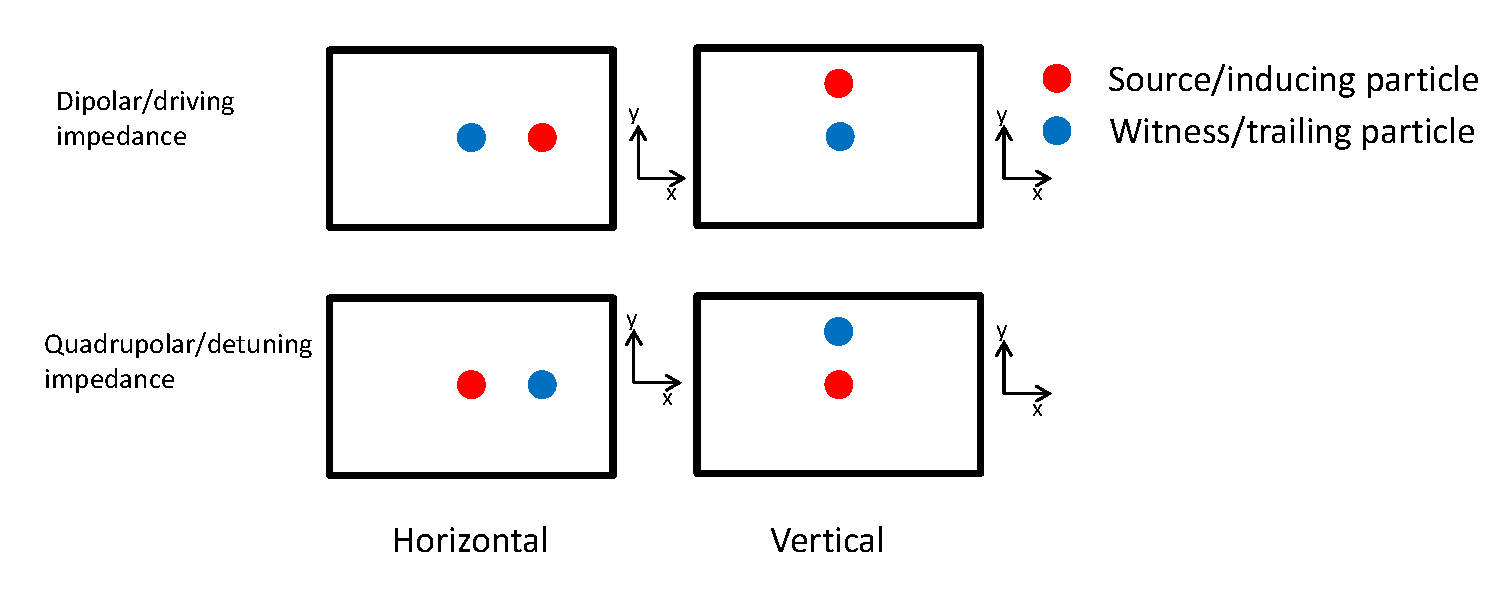
\includegraphics[width=0.9\textwidth]{Wakefields_and_Impedances/figures/impedance-des.pdf}
\end{center}
\caption{The relative displacements of the source and witness particle in the horizontal and vertical planes that identify the dipolar/driving and quadrupolar/detuning impedances.}
\label{fig:trans_imp_disp}
\end{figure}

%\begin{itemize}
%\item{Firstly mention the commonality of frequency dependent material properties - ferrite permeability, permitivitty determined by conductivity/frequency in conductors/dielectrics/skin depth}
%\item{Fourier transform of wakefield into the convolution of the beam current spectrum and the impedance}
%\item{Again Panowsky-Wenzel for impedance}
%\item{Discussion of the transverse impedance - in particular the general definition of an impedance (n-th order current interacting with an m-th order field)}
%\item{Define dipolar/driving and quadrupolar/detuning impedance. In addition constant transverse impedance term}
%\end{itemize}